\chapter{研究问题的核心概念}

为了后续讨论的方便和统一,在本章中,我们给出电子表格的编程模型,在模型描述方面我们借鉴了窦文生等人的经验\cite{dou2017cacheck},并定义单元格类和单元格的公式缺陷这类核心概念\footnote{除额外说明之外,我们用\textit{数值单元格}专指那些单元格里的数值是直接给出而不是计算得来的单元格,用\textit{公式单元格}专指那些单元格里的数值是根据自身公式计算得来的单元格。当然电子表格中也包含其它类型的单元格,如字符串单元格、日期单元格等,由于这些类型不是本文关注的重点,可以都笼统地看成字符串单元格。}。


\section{电子表格的编程模型}
一个电子表格可以被建模成一个集合,其中包含带有表达式的单元格,这些单元格使用二维地址\footnote{我们暂不考虑跨表的情况,将电子表格看成二维的表格结构,本质上三维的建模方式与此类似。}来索引,一个行索引和一个列索引,如 B1 或者 C2。
数值单元格和公式单元格的表达式分别通过纯粹的数值和公式来刻画。
一个公式通过\textit{单元格引用}来引用另一个单元格,单元格引用也是通过被引用的单元格地址来索引。
用$R$来表示单元格引用的集合,$EXP$来表示表达式的集合,$V$表示纯粹数值的集合。
一个公式单元格的表达式 $exp$ 要么是一个纯粹数值($v \in V$)、一个单元格引用($r \in R$)或者一个引用若干个子表达式的公式($\varphi $)。
电子表格中使用的函数包括基本的运算符(例如,“$+$”,“$-$”,“$*$”和“$/$”),以及大量电子表格软件中的内置函数(如 SUM,AVERAGE 和 IF 等)。
一个公式单元格的表达式$exp$可以形式化地表达为:
\begin{definition}
    $ exp =\quad v\quad |\quad r\quad |\quad \varphi (exp_1,\dots,exp_n) $
\end{definition}

我们定义获取一个公式单元格的所有直接引用的单元格的函数 $\sigma(exp)$ ,它返回一个集合,其中包含在该公式中使用到的所有被引用的单元格。
类似于对表达式的描述,函数 $sigma(exp)$ 也可以形式化地表达为:
\begin{definition}
$
\sigma(exp) = 
\left\{
    \begin{aligned}
       & \emptyset & exp \in V; \\
       & \{exp\}     & exp \in R; \\
       & \sigma(exp_1) \cup \dots \cup \sigma(exp_n) & exp = \varphi(exp_1, \dots , exp_n).
    \end{aligned}
\right.
$
\end{definition}

\begin{figure}[tp]    
    \centering
    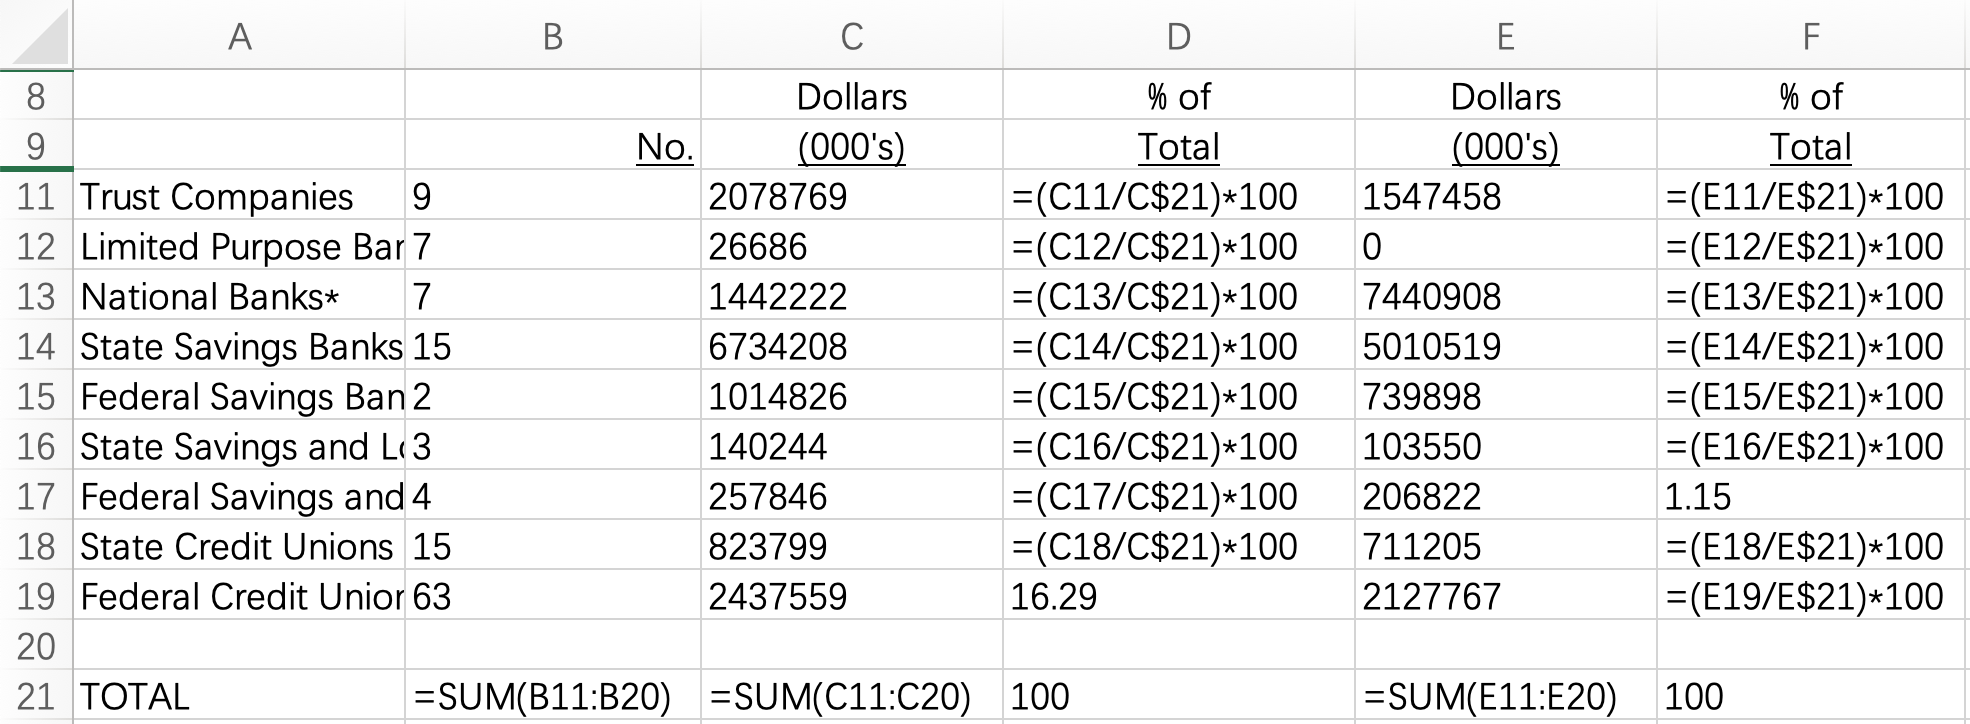
\includegraphics[width=\textwidth]{figure/style-A1.png}
    \caption{截取自EUSES 数据库中的电子表格 summ0602.xls 的工作表summary1201(A1 表示法)}
    \label{figure-A1}
\end{figure}
\begin{figure}[tbp]    
    \centering
    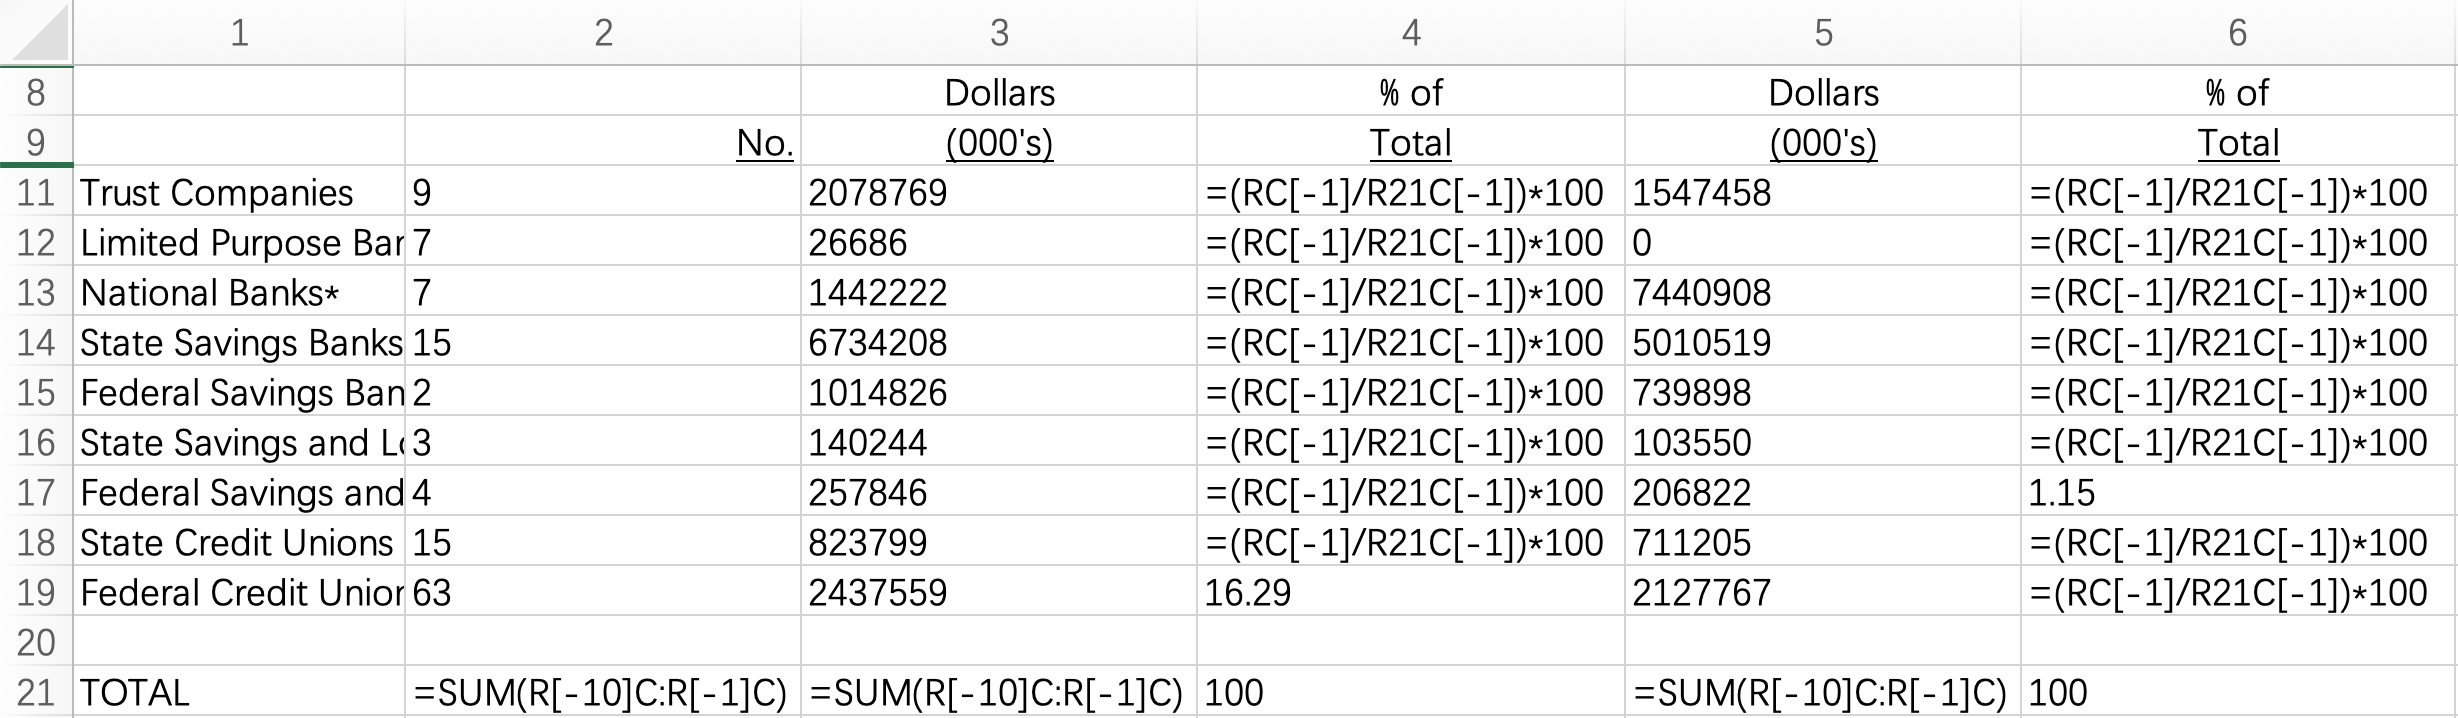
\includegraphics[width=\textwidth]{figure/style-R1C1.png}
    \caption{截取自EUSES 数据库中的电子表格 summ0602.xls 的工作表summary1201(R1C1 表示法)}
    \label{figure-R1C1}
\end{figure}

电子表格软件通常允许两种表达单元格引用的方式,\textit{A1表示法}\footnote{对终端用户更友好}和 \textit{R1C1表示法} \footnote{对程序分析更友好,后面我们在算法设计和分析时采用 R1C1 表示法,但在解释具体的电子表格示例时,依然采用 A1 表示法,这正契合两种表示方式各自的特点} \cite{tan2014bug}。
在特定的引用方式下,还有对被引用单元格所在行和所在列的\textit{绝对引用}和\textit{相对引用}的区别。
绝对引用指向固定行或列的单元格,当该引用被复制到其他单元格,仍然引用相同行或列的单元格。
相对引用表示公式单元格和被引用单元格之间的行或列偏移量,当该引用被复制到其他单元格时,偏移量保持不变,但实际被引用的单元格地址发生了平移变化。

如图 \ref{figure-A1} 所示,该电子表格显示引用的方式是 A1 表示法。
在 A1 表示法中,一个在第 $X$ 列(A,B,\dots,Z,AA,\dots)第 $y$ 行(1,2,\dots)的单元格在行列都是相对引用的情况下表示为 $Xy$(如B5),在行列都是绝对引用的情况下中表示为 $\$X\$y$(如\$B\$5)。
如图 \ref{figure-R1C1} 所示,该电子表格使用 R1C1 表示法,且所有单元格引用都是相对引用。
在 R1C1 表示法中,一个在当前单元格的下方第 $n$ 行(可以是负数,此时表示上方第 $n$ 行)和右侧第 $m$ 列(可以是负数,此时表示左侧第 $m$ 列)的单元格在行列都是相对引用的情况下中表示为 R[$n$]C[$m$](其中,$n$ 或 $m$ 在 $n=0$ 或 $m=0$ 时可以省略,而一个处在第 $n$ 行,第 $m$ 列的单元格在行列都是绝对引用的情况下表示为 R$n$C$m$。
在图 \ref{figure-A1} 和图 \ref{figure-R1C1} 中,单元格 D11 含有两种不同表达形式的公式 =(C11$/$C\$21)$*$100 和 =(RC[-1]$/$R21C[-1])$*$100,这就是绝对引用和相对引用混合使用的例子。

一个有用的观察是:含有相似计算语义的公式单元格通常具有用 R1C1 方式表达的等价表达式。
例如,图 \ref{figure-A1} 中的单元格 D11 中的公式 =(C11$/$C\$21)$*$100 在 R1C1表示法中是图 \ref{figure-R1C1} 中的 =(RC[-1]$/$R21C[-1])$*$100。
图 \ref{figure-R1C1} 也给出了图 \ref{figure-A1} 中其他所有公式对应的 R1C1 表示结果。
我们不难观察出:在 A1 表示法下,从 D11 到 D18 的公式表达式不尽相同,但在 R1C1 表示法下,从 D11 到 D18 的公式表达式完全等价,因此在算法分析和设计时使用后一种表示法更为有利。
我们利用这一观察,从公式表达式中抽取特征来将单元格进行区分,将形式类似的公式吸纳进同一个类中,进而检测出该类中存在的缺陷单元格。

\begin{figure}[tbp]    
    \centering
    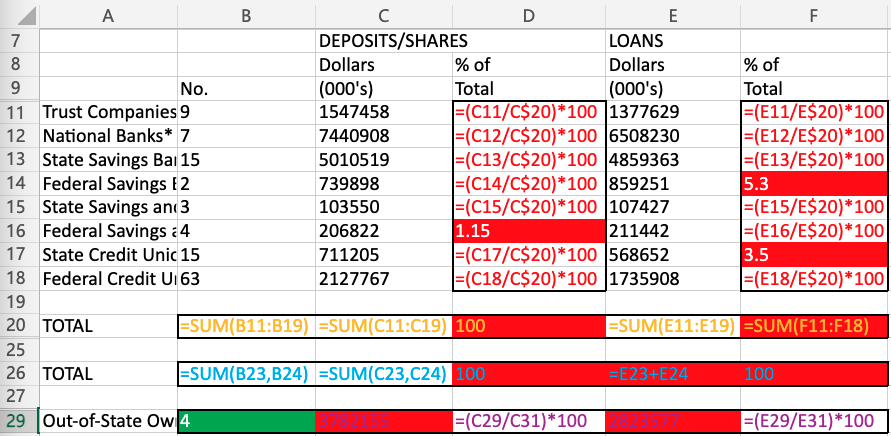
\includegraphics[width=1\textwidth]{figure/figure-3-3.png}
    \caption{电子表格的单元格类和公式缺陷示意图}
    \label{figure-3-3}
\end{figure}


\section{电子表格的单元格类}
我们首先给出在本文中电子表格单元格类的定义:

\begin{definition}
    \textit{单元格类}是单元格的集合,即$Cluster = \{cell_1, cell_2, \dots\}$,其中每个单元格 $cell_i$ 都具有\textit{相似}的\textit{计算语义}。
\end{definition}

要理解单元格类,需要在各类技术中明确其中的两个关键概念:

\begin{itemize}
    \item \textit{计算语义}的概念:能够直接或者间接表明该单元格的计算语义的单元格特征,都可以用来一定程度上表征该单元格的计算语义。例如,直接的特征就是该单元格拥有的公式(但该公式可能有缺陷,未必完全准确地反映该单元格的真实应该表达的计算语义)。间接的特征也存在很多形式,比如,该单元格周围的其他单元格的计算特征,或者该单元格所在的表头字符串信息等,都可以暗示该单元格可能拥有的计算语义。
    \item \textit{相似}的概念:通常刻画相似的方法是量化该单元格与一个单元格集合中其他单元格的计算特征的相似度。比如,可以比较从单元格中抽取出的直接特征和间接特征的相似度的方法,来权衡最终两个单元格的相似度。
\end{itemize}

如图\ref{figure-3-3}所示,从单元格 B20 向左延伸到 F20 的五个单元格都是统计每个单元格上方的若干个单元格的数量和,这五个单元格就天然构成了一个单元格类。他们都具有在相似位置进行求和运算的计算语义,首先单元格 B20、C20 和 E20 拥有完全相同的 R1C1 表示法下的公式表达式,因此可以归为同类;而考虑到单元格 D20 和 F20 的位置,以及 F20 具有的相似公式表达式(区别仅在于引用单元格不尽相同),D20 具有数值 100,这恰好就是单元格 D11 到 D19 的总和,因此也可以归为同类。

在缺乏终端用户的先验知识的前提下,如何定义计算语义,以及如何量化单元格之间的计算语义相似度,正是各类电子表格缺陷检测技术的核心挑战之一\cite{Barowy2018excelint}。
使用识别单元格类作为中间环节的缺陷检测技术,通常会将电子表格中的所有公式单元格和数值单元格进行分类,形成单元格类的集合。最后,利用这些单元格类,在每个类中,进行缺陷检测识别出有问题的单元格。


\section{电子表格的公式缺陷}
在定义“单元格类”概念后,我们来解释何为电子表格的公式缺陷。
同样参考图\ref{figure-3-3},其中总共包含 4 个单元格类(单元格类用字体颜色区分,分别为红、黄、蓝和紫)和 10 个公式缺陷,下面详细分析。
通常,有缺陷的单元格中一定存在\textit{替换}导致的异常,通常是用不合法的子表达式替换了原有的合法子表达式。
这里,我们根据定义 3-1 的表达式结构刻画对公式缺陷进行如下分类。

\subsection{用数值替换的公式缺陷}
在公式单元格中用某个数值常量替换一个子表达式(如单元格引用),但它的同类单元格并没有进行这番替换时,该公式单元格具有的公式缺陷就称为\textit{用数值替换的公式缺陷}。
现实情况下,存在大量用常量替换整个公式的情况,此时公式单元格退化成了数值单元格,使得检测该类缺陷更为困难。
在图\ref{figure-3-3}中,有 8 个单元格具有此类公式缺陷,虽然它们本身都是数值单元格,但它们的确具有计算语义,如单元格 D16,显然它的同列几个公式(从 D11 到 D18)都是用来计算左侧单元格的占比,而 D16 只有一个常量 1.15。
如果将来改动了单元格 C16 的值,那么 D16 显示的数值就不再准确,因此该类公式缺陷应该被修复。

\subsection{用单元格引用替换的公式缺陷}
类似地,我们把一个单元格用一个错误的单元格或者单元格范围替换一个子表达式,然而其它的同类单元格并没有这么替换时,这类单元格的缺陷称为\textit{用单元格引用替换的公式缺陷}。
在图\ref{figure-3-3}中, 单元格 F20 的引用集合$\sigma$(SUM(F11:F18))比起同一行中的其他几个公式缺少了对单元格 F19 的引用。
如果将来在第 19 行添加了新的数据,那么 F20 的计算结果不再准确,因此该类公式缺陷应该被修复。

\subsection{用操作符/函数替换的公式缺陷}
类似地,我们把一个单元格用一个错误的操作符/函数替换一个子表达式,然而其它的同类单元格并没有这么替换时,这类单元格的缺陷称为\textit{用操作符/函数替换的公式缺陷}。
在图\ref{figure-3-3}中,单元格 E26 具有与 B26 和 C26 不同的操作符,E26 使用加法操作,而另外两个公式采用内置函数 SUM 来求和。
如果将来求和的范围扩大了,由于公式形式不同,可能忘记对 E26 的更新,因此该类公式缺陷也该被修复。

\subsection{小结}
上述三类单元格缺陷类型已在真实商业场景下频繁发现\cite{panko2006facing,powell2008critical}。
由于缺陷的类型和变体多种多样,普通终端用户在选用电子表格测试技术时,由于并不预先知道自己的表格中潜在的缺陷类型,难以针对性地选择特定检测技术。
那么基于学习的单元格聚类技术因为天生具有对多种缺陷的适应性,能够把上述各种类型的缺陷单元格都尽可能不遗漏地加入到单元格类中,最后再统一地进行缺陷检测分析。
这对于终端用户来说,是一个容易接受并采纳的电子表格缺陷检测技术方案。